\documentclass{article}
\usepackage{enumerate}
\usepackage{amsmath}
\usepackage{amssymb}
\usepackage{graphicx}
\usepackage{subfigure}
\usepackage{geometry}
\usepackage{caption}
\usepackage{indentfirst}
\usepackage{tikz}

\usepackage{algorithm}
\usepackage{algorithmicx}
\usepackage{algpseudocode}
\renewcommand{\algorithmicrequire}{\textbf{Input:}}
\renewcommand{\algorithmicensure}{\textbf{Output:}}

\geometry{left=3.0cm,right=3.0cm,top=3.0cm,bottom=4.0cm}
\renewcommand{\thesection}{Exercise 8.\arabic{section}}
\title{VE203 Assignment 8}
\author{Liu Yihao 515370910207}
\date{}
\begin{document}
\maketitle

\section{}

By the hint, we can guess that it is about the attack on the Pearl Harbour, and we can find 19 17 19 19, so they are probably ``ATTA" in the word ``attack" .If we make a deeper guess, the list from 19 in the first column and 8 in the fourth column is ``ATTACK PEARL HARBOR". Then I find on the wiki that the attack happened on Dec 7th, and it just fit the other numbers. So the complete message is ``ATTACK PEARL HARBOR DECEMBER SEVEN".

\section{}
$$c=m^e{\rm\ mod\ }n=23^7{\rm\ mod\ }77=23(23-77\times7)^3{\rm\ mod\ }77=23$$

\section{}
Suppose $g^a$, $g^b$ are two elements in $G$
$$g^a\circ g^b=g^{a+b}=g^{b+a}=g^b\circ g^a$$ 

\section{}
$$3^a\equiv 6{\rm\ (mod\ }7)$$
$$3^b\equiv 5{\rm\ (mod\ }7)$$
$$a=3,\ b=5$$
$$5^3\equiv 6^5\equiv 6{\rm\ (mod\ }7)$$
So their common secret key is $6$

\section{}
\begin{enumerate}[i)]
\item
vertices: 6\\
edges: 6\\
degrees: $a_1=2$, $a_2=4$, $a_3=1$, $a_4=3$, $a_5=2$, $a_6=0$
\begin{table}[!h]
\begin{center}
\begin{tabular}{c|cccccc}
	 &$a_1$&$a_2$&$a_3$&$a_4$&$a_5$&$a_6$\\ \hline
$a_1$&	0  &  1  &  0  &  1  &  0  &  0  \\
$a_2$&	1  &  0  &  1  &  1  &  1  &  0  \\
$a_3$&	0  &  1  &  0  &  0  &  0  &  0  \\
$a_4$&	1  &  1  &  0  &  0  &  1  &  0  \\
$a_5$&	0  &  1  &  0  &  1  &  0  &  0  \\
$a_6$&	0  &  0  &  0  &  0  &  0  &  0  \\
\end{tabular}
\end{center}
\end{table}
\newpage
\item
vertices: 6\\
edges: 12\\
degrees: $a_1=6$, $a_2=5$, $a_3=0$, $a_4=3$, $a_5=5$, $a_6=5$
\begin{table}[!h]
\begin{center}
\begin{tabular}{c|cccccc}
	 &$a_1$&$a_2$&$a_3$&$a_4$&$a_5$&$a_6$\\ \hline
$a_1$&	2  &  3  &  0  &  1  &  0  &  0  \\
$a_2$&	3  &  0  &  0  &  1  &  1  &  0  \\
$a_3$&	0  &  0  &  0  &  0  &  0  &  0  \\
$a_4$&	1  &  1  &  0  &  0  &  1  &  0  \\
$a_5$&	0  &  1  &  0  &  1  &  0  &  3  \\
$a_6$&	0  &  0  &  0  &  0  &  3  &  2  \\
\end{tabular}
\end{center}
\end{table}
\item
vertices: 9\\
edges: 10\\
degrees: $a_1=2$, $a_2=2$, $a_3=2$, $a_4=0$, $a_5=2$, $a_6=3$, $a_7=2$, $a_8=4$, $s_9=5$
\begin{table}[!h]
\begin{center}
\begin{tabular}{c|ccccccccc}
	 &$a_1$&$a_2$&$a_3$&$a_4$&$a_5$&$a_6$&$a_7$&$a_8$&$a_9$\\ \hline
$a_1$&	0  &  0  &  0  &  0  &  0  &  1  &  0  &  0  &  1  \\
$a_2$&	0  &  0  &  0  &  0  &  0  &  0  &  1  &  0  &  1 \\
$a_3$&	0  &  0  &  0  &  0  &  0  &  1  &  0  &  1  &  0  \\
$a_4$&	0  &  0  &  0  &  0  &  0  &  0  &  0  &  0  &  0  \\
$a_5$&	0  &  0  &  0  &  0  &  0  &  0  &  0  &  0  &  0  \\
$a_6$&	1  &  0  &  1  &  0  &  0  &  0  &  1  &  0  &  0  \\
$a_7$&	0  &  1  &  0  &  0  &  0  &  1  &  0  &  0  &  0  \\
$a_8$&	0  &  0  &  1  &  0  &  0  &  0  &  0  &  0  &  3  \\
$a_9$&	1  &  1  &  0  &  0  &  0  &  0  &  0  &  3  &  0  \\
\end{tabular}
\end{center}
\end{table}
\end{enumerate}

\section{}
\begin{enumerate}[i)]
\item
$$V_1={a,c},V_2={b,d,e}$$
So it is bipartite.
\item
Since $b,f,c$ forms a triangle, it is not bipartite.
\item
Since $b,e,f$ forms a triangle, it is not bipartite.
\end{enumerate}

\section{}
\begin{enumerate}[i)]
\item \ 
\\
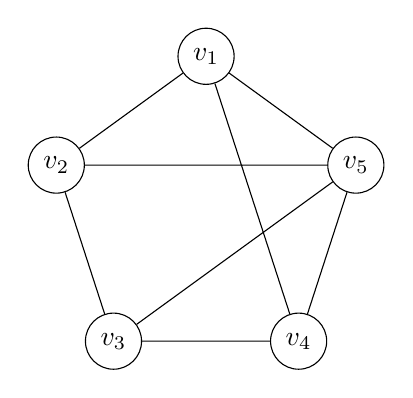
\begin{tikzpicture}[scale=2]
\tikzstyle{every node}=[draw,shape=circle];
\foreach \i in {1,...,5}
{
\path (18+72*\i:1cm) node (v\i) {$v_\i$};
}
\draw
(v1) -- (v2)	(v1) -- (v4)	(v1) -- (v5)
(v2) -- (v3)	(v2) -- (v5)
(v3) -- (v4)	(v3) -- (v5)
(v4) -- (v5);
\end{tikzpicture}
\item \ 
\\
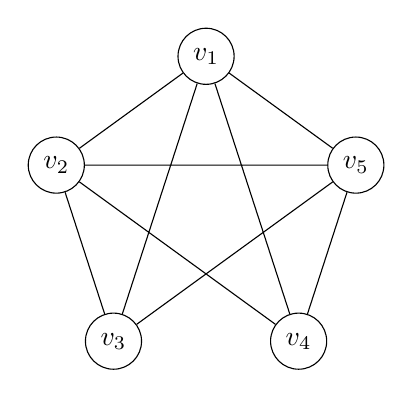
\begin{tikzpicture}[scale=2]
\tikzstyle{every node}=[draw,shape=circle];
\foreach \i in {1,...,5}
{
\path (18+72*\i:1cm) node (v\i) {$v_\i$};
}
\draw
(v1) -- (v2)	(v1) -- (v3)	(v1) -- (v4)	(v1) -- (v5)
(v2) -- (v3)	(v2) -- (v4)	(v2) -- (v5)
(v3) -- (v5)
(v4) -- (v5);
\end{tikzpicture}
\item \ 
\\
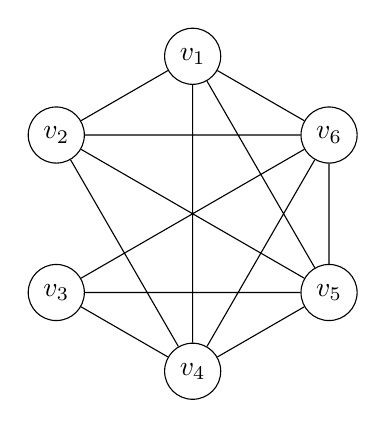
\begin{tikzpicture}[scale=2]
\tikzstyle{every node}=[draw,shape=circle];
\foreach \i in {1,...,6}
{
\path (30+60*\i:1cm) node (v\i) {$v_\i$};
}
\draw
(v1) -- (v2)	(v1) -- (v4)	(v1) -- (v5)	(v1) -- (v6)
(v2) -- (v4)	(v2) -- (v5)	(v2) -- (v6)
(v3) -- (v4)	(v3) -- (v5)	(v3) -- (v6)
(v4) -- (v5)	(v4) -- (v6)
(v5) -- (v6);
\end{tikzpicture}
\end{enumerate}

\end{document}
